\chapter{级联随机蕨回归框架下的物体六维位姿估计}

\section{概述}

在工业装配现场,为了实现生产过程的高效自动化,很多场合需要对工业零件或是一般物体进行自动化抓取或者放置。目前大多数场合下实现物体的自动化抓取以及放置采取的措施都是通过将被抓取或者放置的物体固定在一些具有非常高精度的位置上,并事先调试好固定代码来控制机械臂等执行机械进行操作。但这个方法需要大量的人力资源对工业现场进行部署,同时物体的位姿估计算法也须要针对每一个零件进行特殊的设计,大大降低了工业生产效率。因此下文将通过讨论一个新颖的物体位姿估计算法,来克服上述几个工业现场存在的问题。

本章的主旨是借鉴人脸特征点定位这个研究领域取得的杰出成果,提出一个更加通用高效的物体六维位姿估计算法框架。通过重新设计全新特征描述,使算法在深度图像上具有较高的信噪比,同时具备一定的尺度不变性。在第二章中已经给出了随机蕨算法的核心功能,本文将借助随机蕨回归算法,将其用于物体的六维位姿估计。其中,提出的新物体位姿估计算法框架需要大量的标记数据进行回归模型的训练,而第三章内容通过仿真深度相机可以在短时间内提供大量的此类数据,为该算法的研究提供了重要支撑。最后本文将进一步探讨遮挡情况下,利用大噪声干扰下的随机蕨回归算法进行异步位姿回归,从而克服遮挡情况对物体位姿回归的影响。

本章结构安排如下:节4.2内容主要讨论深度图像上的新特征设计,以及新特征的哈希处理。节4.3给出了物体位姿估计的主要流程框架以及框架中一些重要的实现细节。节4.4则进一步给出了如何将随机蕨算法改造后应用于遮挡情况下的物体位姿估计。最后通过实验逐一验证上述算法的可行性以及高效性。

\section{深度图像上的特征设计}

类似于SIFT、SURF、FAST等经典的特征描述一般都是针对RGB图像或者灰度图像进行设计的,这些特征描述能够反映出图像特征点周围的色彩或者纹理信息。这些特征点描述一般而言具有相对较高的计算复杂度,从而能够携带非常丰富的信息,因此具有非常好的稳定性。但在物体的位姿估计应用中这些特征描述就相对显得比较乏力。这些特征描述无法携带物体的深度信息,在描述深度图像中的特征点的时候不能够具有尺度不变性。也就是说对于物体的同一个特征点,不同的距离下,这些特征描述方法得到的结果都是不一样的。而我们通常希望在描述一个物体的同一个特征点的时候,不管该特征点距离深度相机的远近,都应该具有相同的特征描述。本文将主要针对这个问题介绍一种具有尺度不变性的全新特征描述。

\subsection{深度图像块的特征描述} % 

深度图像和传统RGB图像最本质的区别在于深度图像中每一个像素值反应的是这个位置的物体距离深度相机的距离,而不是这个物体的纹理信息。因此在对深度图像中的某一个位置进行特征描述的时候,应该充分考虑到这个位置本身的深度值,或者说在该处进行特征描述的过程应该是和该位置的深度值成一定函数关系的,如下式所示:
\begin{equation}
	F=D(I(x,y))
\end{equation}
其中$F$表示特征描述,$I$表示深度图像,$I(x,y)$表示在深度图像坐标$(x,y)$处对应点的深度值,$D(\cdot)$特征描述的具体表达形式。

另一方面,考虑到在物体位姿估计过程中,特别是针对工业现场下的物体位姿估计,物体都是具有相对稳定的结构,因此在进行一个物体的位姿描述的时候,不应该只局限于描述物体上某一个点周围的纹理信息,而应该考虑到将整个物体的概况整体描述进特征里。也就是说,在深度图像上进行特征描述的过程,应该是针对一个局部深度图像块的,这个深度图像块的大小根据透视变换的几何性质应该正比于该位置的深度值平方:
\begin{equation}
\begin{aligned}
	& D(I(x,y))\equiv{D_\Delta}(I(x,y)) \\
	& \Delta\propto{I^2(x,y)}
\end{aligned}
\end{equation}

这一点应该类似于目前较为成熟的人脸特征点定位中的特征描述。在对人脸特征点进行定位过程中,由于人脸具有非常强的对称性,脸部很多地方存在局部相似,如果不考虑整个人脸的整体信息进行直接定位回归的话会导致算法极易陷入局部极小值而失败。目前人脸特征点定位领域中表现最好的算法采用的特征描述称为差值形状索引特征(Interpolated shape-indexed features)\cite{burgos2013robust}。如图4-1所示,
\begin{figure}[htb]
	\centering 
	% \includegraphics[width=\textwidth]{./Pictures/test.jpg} 
	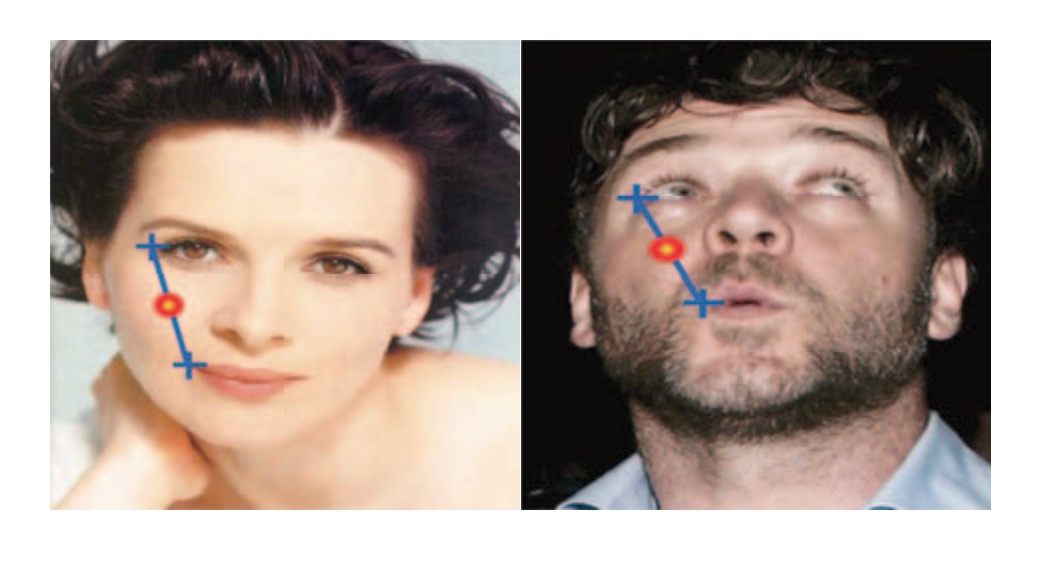
\includegraphics[width=0.8\textwidth]{./mypic/人脸特征描述方法.jpg} 
	\caption{人脸特征描述方法中的差值形状索引特征} 
\end{figure}
图中人脸形状由人脸特征点列构成(图中十字点,为了方便阐述仅画出两个),任意取特征点列中的两个点作为基础点,给一个随机比例差值可以得到一个新的点。所有这些通过差值得到的点像素构成一个集合,两两像素值做差便得到了基础特征描述库。可以看出,在人脸特征点定位中用到的特征描述具有非常简洁的形式:
\begin{equation}
	f_{p_1,p_2}(I)=I(p_1)-I(p_2)
\end{equation}
但事实证明,这样简洁的特征描述确实能够很好地表达出人脸面部特征,并能以此回归出非常精准的特征点定位结果。本文认为这样的特征描述之所以能有非常好的表达能力,关键在于基础特征库的生成是通过整体特征点差值得到的。这一步骤不仅仅能将人脸整体的概况信息包含进去,同时也能够通过差值的方式反映出人脸局部的一些结构信息,实现了从概况到细节的所有信息的融合。因此,本文受该特征描述的启发,结合深度图像本身的特点提出一种全新的特征描述方式。
\begin{figure}[htb]
	\centering 
	% \includegraphics[width=\textwidth]{./Pictures/test.jpg} 
	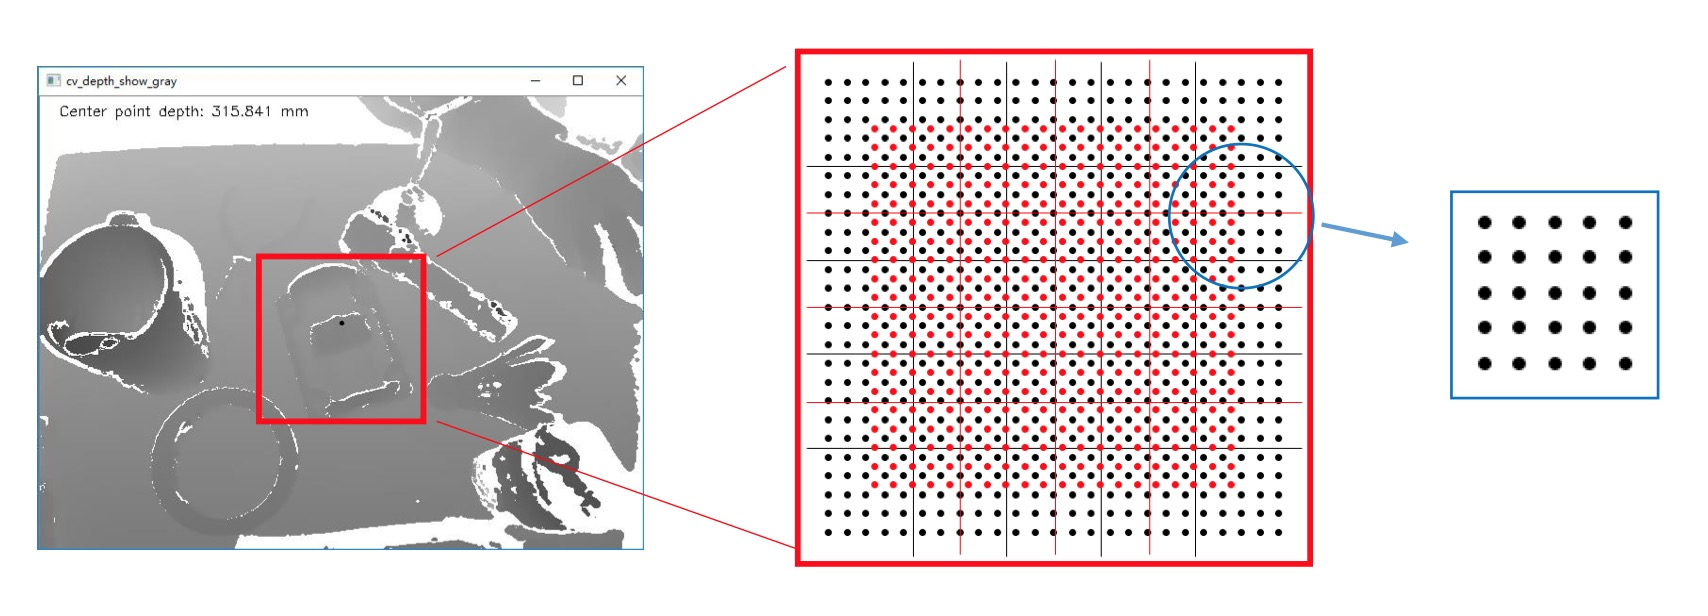
\includegraphics[width=\textwidth]{./mypic/物体位姿估计特征描述方法.jpg} 
	\caption{物体位姿估计特征描述方法} 
\end{figure}

在给定物体的大致位置后(深度图像中该物体的中心点像素坐标),首先由公式(4-2)给出的关系确定特征描述块的大小,使得特征描述框能够覆盖整个物体。实际算法部署过程中,会事先人为标注一个标准距离$d_0$下特征描述框的大小$S_0$,当遇到新场景下实际物体距离为$d'$时,可以直接计算出新的特征描述框大小:
\begin{equation}
	S'=\left(\frac{d'}{d_0}\right)^2\cdot S_0
\end{equation}

下一步须要将得到的特征描述框进行划分。首先将其均分成5*5个子方块,每个子方块相互紧挨覆盖整个特征描述框,如图4-2中间黑线划分方式。然后再在原始特征描述框的中部取4*4个子方块,每个子方块的大小与先前黑线划分得到的子方块大小相同,并且这16个子方块中的每一个方块都位于黑线划分得到的其中4个方块的交界处。这样总共可以得到41个特征描述框子区域。

得到上述这41个子区域之后,将这41个子区域进行平均采样25个像素点(如图4-2最右侧所示),第$A_k$个子区域上的点记为$\{d_{k_1},d_{k_2},...,d_{k_n}\}$,总共可以得到1025个特征样本点。但这些像素点的深度值信息过于简单,不能直作为特征,需要进一步处理。对于每一个子区域上的25个像素点,我们计算其深度均值$\bar{d}_k$,并将这25个像素点的深度值减去$\bar{d}_k$。这样在每一个子区域中,串联所有的深度值之差以及该深度均值可以得到一个26纬度的子特征,总共可以得到1066维度的特征。然后继续计算上述所有子区域中采样得到的深度均值的均值:
\begin{equation}
	\bar{d}_{all}=\frac{1}{41}\sum_{k=1}^{41} \bar{d}_k
\end{equation}
再将这41个子区域的均值减去$\bar{d}_{all}$得到另外25维度特征,最后加上$\bar{d}_{all}$本身,一共可以得到1092维度的特征描述。

通过这样将整个特征描述区域进行拆分采样,最后通过相互取均值做差的方式进行特征整合描述,可以充分描述出整个区域上的深度分布情况,同时也将局部特征信息包含进特征描述中形成一个具有非常完备的特征描述形式。并且由于特征描述区域大小是通过实际的深度值计算得到的,因此这种特征描述方式具有很好的尺度不变特性。

\subsection{特征哈希处理} % 

为了使特征描述有更高的信噪比,需要对特征进行降维或者哈希化处理。本文借鉴了F. Shen等人在2015年CVPR中提出的监督学习下的哈希算法\cite{shen2015supervised},通过适当简化其算法过程,提高其算法效率的同时保持其哈希处理的高信噪比优势。

假设存在$n$个特征样本$X=\{x_i\}^{n}_{i=1}$,并且期望将其在监督学习下降维得到长度为$L$的二进制编码$B=\{b_i\}^{n}_{i=1}\in\{-1,1\}^{L\times n}$来代替它,其中$b_i$表示$x_i$的第$i$列二进制码。同时假设在线性分类情况下,有如下式所示的多分类问题:
\begin{equation}
	y=G(b)=W^{\top}b=\left[w_1^\top,...,w_c^\top\right]^\top
\end{equation}
其中$w_k\in \Re^{L\times 1},k=1,...,C$为第$k$类分类向量,$y\in \Re^{C\times 1}$为类别标签向量。显然,上述问题可以等价于求解下式所示的优化问题:
\begin{equation}
\begin{aligned}
	& \min_{B,W,F} \sum_{i=1}^n L\left(y_i,W^\top b_i\right)+\lambda \|W\|^2 \\
	& \ s.t. \  b_i=sgn\left(F(x_i)\right),i=1,...,n.
\end{aligned}
\end{equation}
这里$L(\cdot)$为损失函数,$\lambda$为正则参数,$Y=\{y_i\}_{i=1}^n\in\Re ^{C\times n}$为真值矩阵。这里将二进制限制放宽为连续函数$F(x)$,同时引入二进制损失项,可以得到最后的优化问题如下:
\begin{equation}
\begin{aligned}
	& \min_{B,W,F} \sum_{i=1}^n L\left(y_i,W^\top b_i\right)+\lambda \|W\|^2 + \nu\sum_{i=1}^n \|b_i-F(x_i)\|^2     \\
	& \quad\quad\quad\quad\quad\quad\quad s.t. \  b_i\in\{-1,1\}^L.
\end{aligned}
\end{equation}

考虑到计算效率,本文采用线性学习算法来直接构建$F(x)$:
\begin{equation}
\begin{aligned}
	& \quad\quad\quad\quad\quad\quad F(x)=P^\top\phi(x) \\
	& \phi(x)=\left[\exp(\frac{\|x-a_1\|^2}{\sigma}),...,\exp(\frac{\|x-a_m\|^2}{\sigma})\right]
\end{aligned}
\end{equation}
这里$\{a_j\}_{j=1}^m$是从训练样本里随机选择的$m$个锚点。接下来将取$L_2$作为损失函数,分为3步对该问题进行求解:G-Step,F-Step,B-Step。
\begin{itemize}
\item G-Step: 固定$B$,可以以最小二乘形式得到$W$:
\begin{equation}
	W=(BB^\top+\lambda I)^{-1}BY^\top
\end{equation}
\item F-Step: 固定$B$,可以得到$P$:
\begin{equation}
	P=\left(\phi(X)\phi^\top(X)\right)^{-1}\phi(X)B^\top
\end{equation}
\item B-Step: 固定除$B$之外的所有变量,采用DCC算法(discrete cyclic coordinate descent method),可以对$B$进行逐位求解:
\begin{equation}
	B: z=sgn(q-B'^\top W'\nu)
\end{equation}
\end{itemize}
其中$z^\top$表示$B$的第$l$行,$B'$表示矩阵$B$除开$z$后的子矩阵,$q^\top$表示$Q=WY+\nu F(X)$的第$l$行,$Q'$表示矩阵除开$q$后的子矩阵,$\nu^\top$表示$W$矩阵的第$l$行,$W'$表示$W$矩阵除开$\nu$后的子矩阵。

在实际应用过程中,通过不断迭代循环上述三个步骤,代入计算$W$,$P$以及$z$,便可逐步收敛,得到最后的哈希码$B$。

但由于在这个算法中锚点的计算会消耗大量的计算资源,为了提高回归算法的效率,本文舍弃锚点的选取,直接采用原始特征信息作为训练的数据,并同时采用回归目标值作为学习目标直接带入算法,不再将回归目标值映射到分类问题上进行处理。通过上述步骤就可以得到下文所需要用到的用于位姿回归拟合的最终哈希特征。

\section{针对位姿估计的级联回归框架设计}

在传统级联回归框架中,所有级联层之间的功能都是一样的,包括具有完全相同的回归拟合器,也包括完全相同的回归目标。例如,在目前表现最优秀的人脸特征点定位算法中\cite{chen2014joint},采用改进的随机森林作为回归器,回归目标为每一级回归器当前的特征点坐标与真值之间的偏差。并且,在训练每一级回归器的时候用到的回归器训练参数也都是完全一致的,如图4-3所示。

\begin{figure}[htb]
	\centering 
	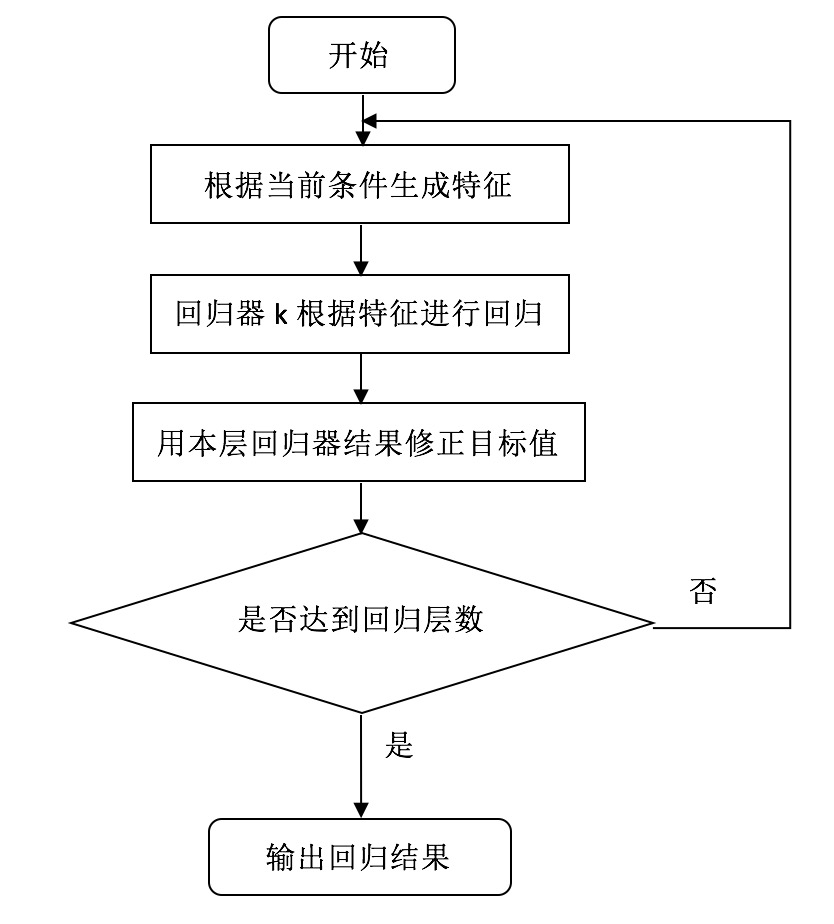
\includegraphics[width=0.6\textwidth]{./mypic/经典级联回归算法流程图.jpg} 
	% \includegraphics[scale=1.0]{./Pictures/test.jpg} 
	\caption{经典级联回归算法流程图} 
\end{figure}

但是在物体的位姿估计问题下,需要回归的目标并不是单纯的某些像素值在图像上的坐标,而是比较抽象的物体的六维空间朝向以及空间坐标。这些抽象的回归目标不能在图像上得到直接的反馈,这就会导致下面这样一个问题:
\begin{itemize}
\item 如果采用各级回归模型都完全一致的级联回归框架,并且每一级的回归器训练目标都直接为物体的当前六维位姿。那么将有如下回归优化目标:
\begin{equation}
\begin{aligned}
	& R^t=\arg \min_R \sum_i \|\hat{S}_i-(S_i^{t-1}+R(x_i,S_i^{t-1}))\|^2. \\
	& S:\{dx,dy,dz,d\theta_x,d\theta_y,d\theta_z\}
\end{aligned}
\end{equation}
其中$R$表示各级的回归拟合器,$S_i$表示当前第$i$级物体的六维位姿,$\hat{S}_i$表示位姿的真值,$x_i$表示当前特征描述框。

结合上一节所述,可以很明显看出,在每一级的位姿估计结果$S_i$更新迭代过程中,至少有这三个维度的更新迭代是没有意义的:$\{d\theta_x,d\theta_y,d\theta_z\}$。也就是说,每当一级回归器得到了回归结果之后,虽然可以更新目标物体的当前位姿,但是目标物体当前的位姿对下一级的回归所需要的特征描述所需要的前提是过饱和的。因为按照上节所述的特征描述方法,仅仅需要得知当前物体在深度图像中的质心像素位置即可,也就是仅仅需要$S$中的前三个空间坐标$\{dx,dy,dz\}$。这样一来,如果级联回归框架中每一级都采用完全相同的回归目标的话,就会产生极大的计算资源浪费,大大降低算法的效率,同时回归目标维度的增加也会大大提高回归器训练所需要的时间,甚至可能导致回归器无法得到可靠的回归结果。
\end{itemize}

为了解决上述问题,本文考虑将原始的级联回归框架拆分成两部分,第一部分用于回归物体的质心空间坐标,第二部分用于回归物体的欧拉角位姿。其中第一部分中,由于物体质心空间坐标可以由第三章中的投影关系给出其与深度图像中像素位置的对应关系,这一部分的回归问题可以转化为标准级联回归问题。而第二部分的回归问题较为复杂,是无法转化为级联回归问题的。但得益于第一部分与第二部分的耦合,如果在第一部分问题得到较好的解决情况下,也就是一旦物体的质心空间位置已经得到了较好的估计,在此基础上再进行物体的空间姿态估计将变为地较为容易,回归目标的复杂度也大大降低。因此,可以考虑使用一个相比质心空间坐标回归器稍微强一点的回归拟合器对物体的欧拉角位姿进行直接拟合。

最后将第一部分的基础级联回归器与第二部分的强回归拟合器按先后顺序再次级联,便可以得到物体位姿估计问题下的最终级联回归算法框架,如流程图4-4所示。

\begin{figure}[htb]
	\centering 
	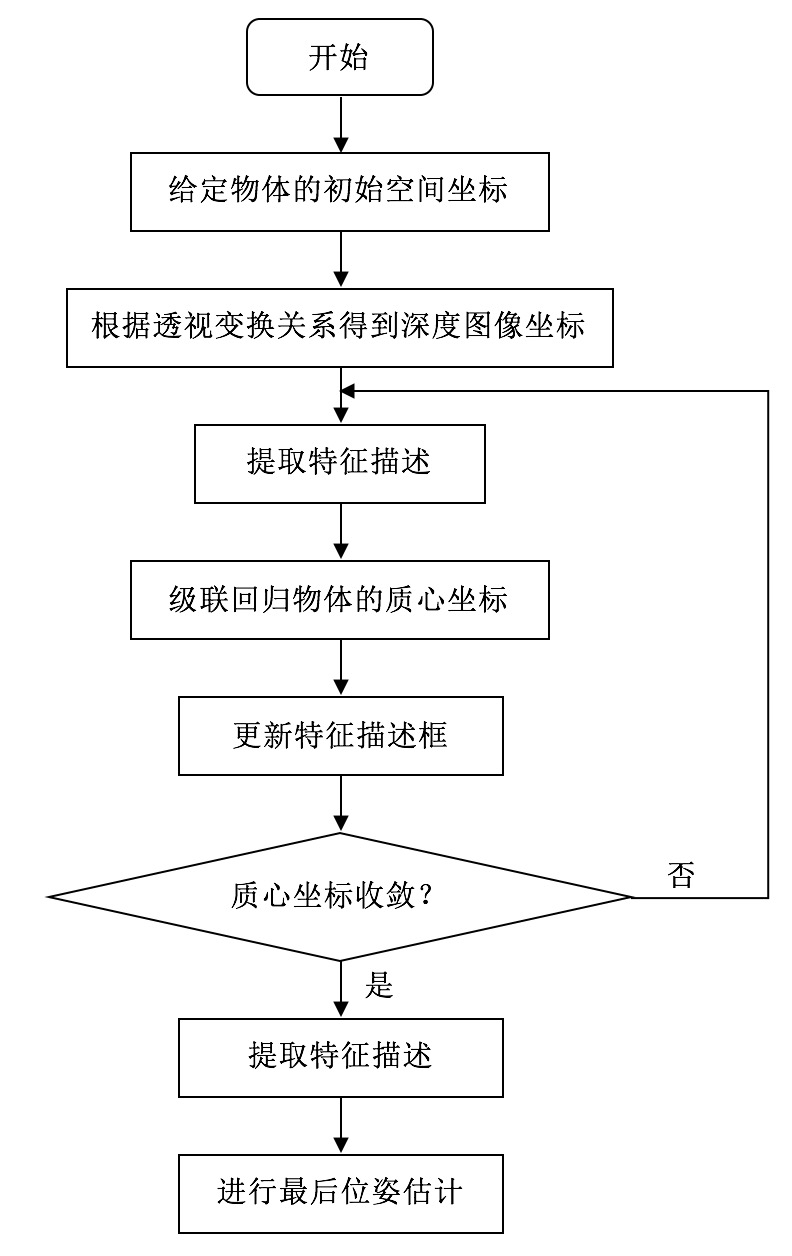
\includegraphics[width=0.6\textwidth]{./mypic/复合式级联回归框架的流程图.jpg} 
	% \includegraphics[scale=1.0]{./Pictures/test.jpg} 
	\caption{复合式级联回归框架的流程图} 
\end{figure}


\section{遮挡情况下的物体位姿估计} % 如何估计物体的被遮挡情况

复杂环境下的物体位姿估计一直以来都是物体位姿估计领域一个重要的难点。当物体在杂乱的环境中,或者工业现场一些零件的堆放过于散乱,会出现物体或者零件被遮挡的情况。结合上文中的特征描述方法,不难得到,一旦物体被局部遮挡,特征描述就会受到极大的干扰。

\begin{figure}[htb]
	\centering 
	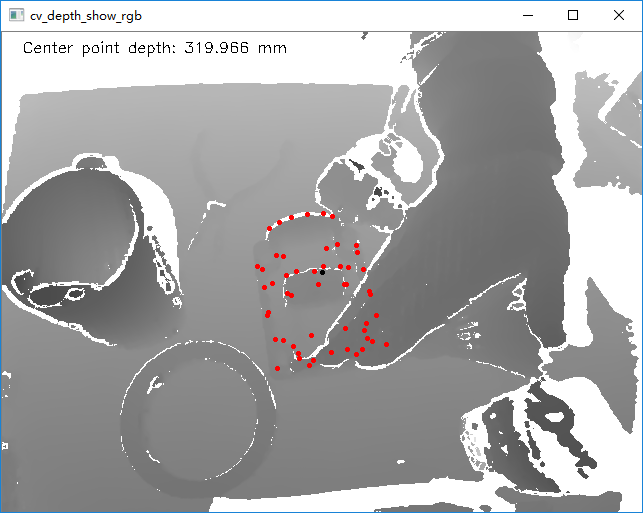
\includegraphics[width=0.5\textwidth]{./mypic/物体存在被遮挡的情况.png} 
	% \includegraphics[scale=1.0]{./Pictures/test.jpg} 
	\caption{物体(红色点区域)被遮挡的情况示意图} 
\end{figure}

如图4-5所示,物体被遮挡将直接导致特征基础库中的像素值完全失去可信度,并且当这些被污染的特征传入后续的随机蕨算法中时,会大大干扰随机蕨算法的最后结果,导致最后物体位姿估计结果发生较大的偏差。因此,本文考虑引入第二章内容所讲的大噪声干扰下的随机蕨算法,利用其掩码的性质来克服物体被遮挡后的位姿回归问题。

由于掩码机制的存在,特征降维操作将不再适用此处,因为如果采用4.2.2节中所用的特征降维方法,经过中间的迭代步骤,会导致最后的哈希特征所有维度都会被污染。而经过实验验证,如果采用未降维的特征作为最后位姿估计的特征,其对应的特征掩码是可以被估计出来的。

在位姿估计这个问题下,要对特征掩码进行预测首先要先对物体的被遮挡情况进行估计。选取经典的随机蕨分类器,以节4.2.1中所述的特征描述作为该分类器的输入,以特征描述区域上的1025个采样点被遮挡情况作为输出,并利用第三章中提到的仿真环境给出的大量有真值标注的数据进行分类器训练,就可以得到我们所需要的掩码估计初步结果。如下式所示:
\begin{equation}
\begin{aligned}
	& M: \left[m_1,m_2,...,m_1025\right]^\top
	& M_i=Classifier_i(F)\in[0,1]
\end{aligned}
\end{equation}

上式中得到的$M_i$在实际计算过程中不能完全取值到严格的0(意味该采样点被遮挡)或者1(意味该采样点为被遮挡),最后的结果是概率化的表达。之后,由于最终的1092维特征所有的维度都是通过这些采样点相互计算得到,因此这1092维特征可以用如下公式来计算其相应的置信度掩码:
\begin{equation}
	W=weight(M)=\frac{\sum M_i\cdot relevant(i)}{S}
\end{equation}
其中,$W$为最后的特征置信度掩码$relevant(\cdot)$函数用来表示该采样点与当前特征维度的相关度,$S$表示当前采样点用到的计算数,例如当前特征维度需要由$k$个基础采样点计算得到,则此处$S$取值就为$k$。当然,由于在本文中的特征描述具有固定的特性,此处$relevant(\cdot)$函数的计算其实可以通过预先计算得到,通过查表的方式得到,从而可以提高算法的效率。

注意上文得到的最后的特征置信度掩码最后的表现形式也是概率化的。有了特征描述以及其对应的特征置信度掩码后,就可以套用本文节2.3中阐述的改进后的随机蕨回归算法代替原先位姿估计框架中的基础随机蕨回归算法,得到可以应对遮挡情况下的物体位姿估计方法。图4-6为有遮挡情况下的物体位姿级联回归框架流程图。

\begin{figure}[htb]
	\centering 
	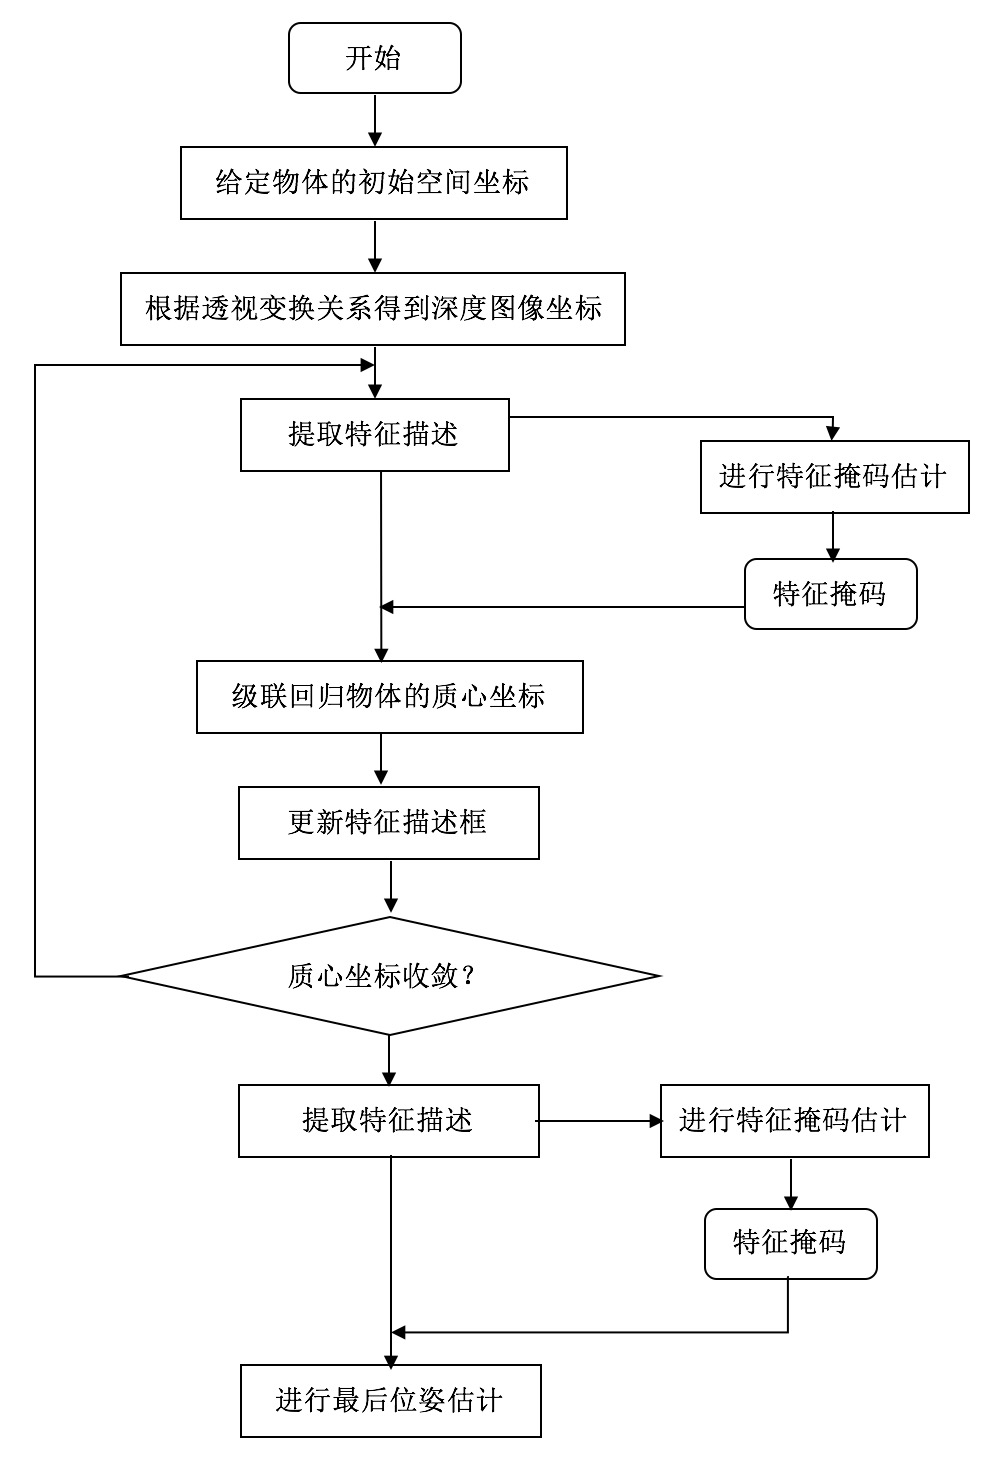
\includegraphics[width=0.75\textwidth]{./mypic/有遮挡情况下的物体位姿级联回归框架流程图.jpg} 
	% \includegraphics[scale=1.0]{./Pictures/test.jpg} 
	\caption{有遮挡情况下的物体位姿级联回归框架流程图} 
\end{figure}


\section{物体检测与物体位姿估计的结合}

前文所述的物体位姿估计算法框架的前提是需要被测物体具有一个较为理想的初始空间坐标。而通常情况下,这个初始空间坐标是不存在的,因此本文提出一种简洁的办法来解决这个问题。

物体的初始空间坐标映射到深度图像中为一个像素点位置,因此给出初始空间坐标本质上可以等价于深度图像上的物体检测问题。物体检测问题通常情况下不外乎物体的特征描述以及一个标准的分类问题。注意到本文在节4.2中提出的特征描述具有非常好的信息表达能力,同时随机蕨算法本身又是一个非常强大的分类器算法。因此可以直接利用本文提出的特征描述,附加一个简单的随机蕨分类器作为物体检测模块。

利用上述方法进行物体检测有一个很自然的特点,就是物体检测与位姿估计所用的特征描述完全一致。这也意味着当物体在深度图像中被检测到时,不需要再重新计算一边特征描述用于位姿估计,从而大大提高算法整体的效率。这个特性是传统方法所不具备的,传统方法往往将物体检测与物体位姿估计两者的特征描述分开设计,效率极低。

本文采用的物体检测采用最基本的滑动窗口方式进行,由于特征描述本身具有一定的描述范围,并且在一个深度情况下只可能存在一个被测物体,因此滑动窗口只需要设置一层,并且按照一定的间隔排布即可,如图4-7所示。

\begin{figure}[htb]
	\centering 
	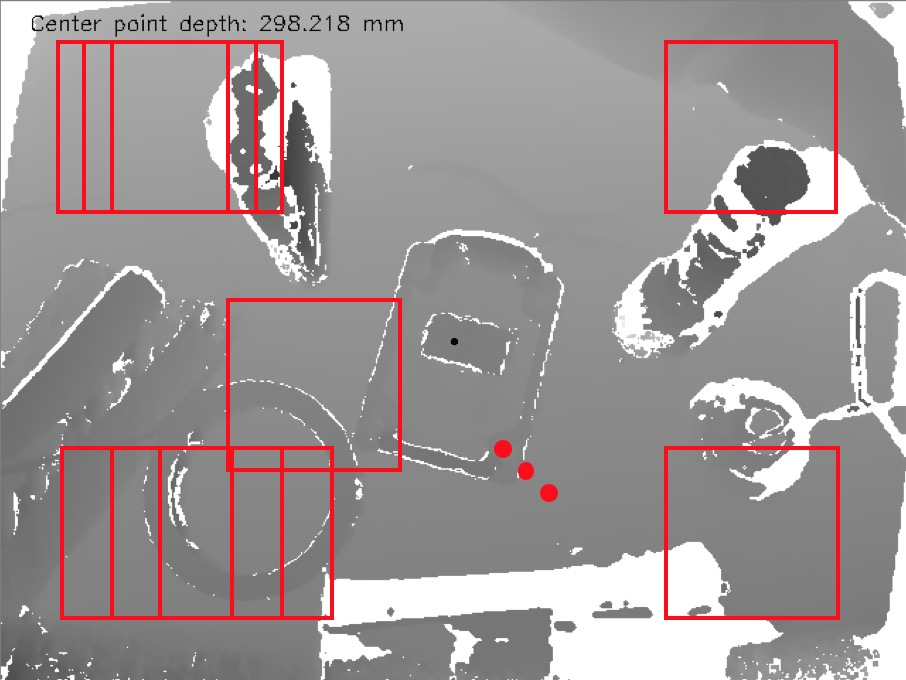
\includegraphics[width=0.7\textwidth]{./mypic/滑动窗口示意图.jpg} 
	% \includegraphics[scale=1.0]{./cyk/test.jpg} 
	\caption{滑动窗口示意图} 
\end{figure}
通过该方法检测到物体的初始状态之后便可以直接作为物体位姿估计算法的初始条件进行后续位姿估计。

\section{实验结果与分析} % 物体检测放在这里讲

\subsection{利用物体位姿特征进行物体检测实验}

本文实验过程中采用的深度相机为Intel公司生产的RealSense SR300系列深度相机,其具备分辨率为640*480大小的红外深度传感器,通过USB接口可以方便获取其深度图像数据。通过人为随机移动该深度相机,使其围绕被检测物体,在此期间持续采集深度图像数据作为本实验的数据来源。此方法下,可以保证物体每一帧都存在于深度图像中,并且有位姿各异的情形。实验中,定义查准率 (precision) 作为评估物体检测能力的好坏。查准率$P$为物体检测器检测到目标人的帧数占所采集到的总帧数的百分比。

如图4-8所示,本文一共对4种物体进行了试验,每一种物体采集了约1500帧深度图像数据,采用经典随机蕨算法作为物体分类器,滑动窗口步长设为对应特征描述区域宽度的一半,得到具体如表4-1所示结果。
\begin{figure}[htb]
	\centering 
	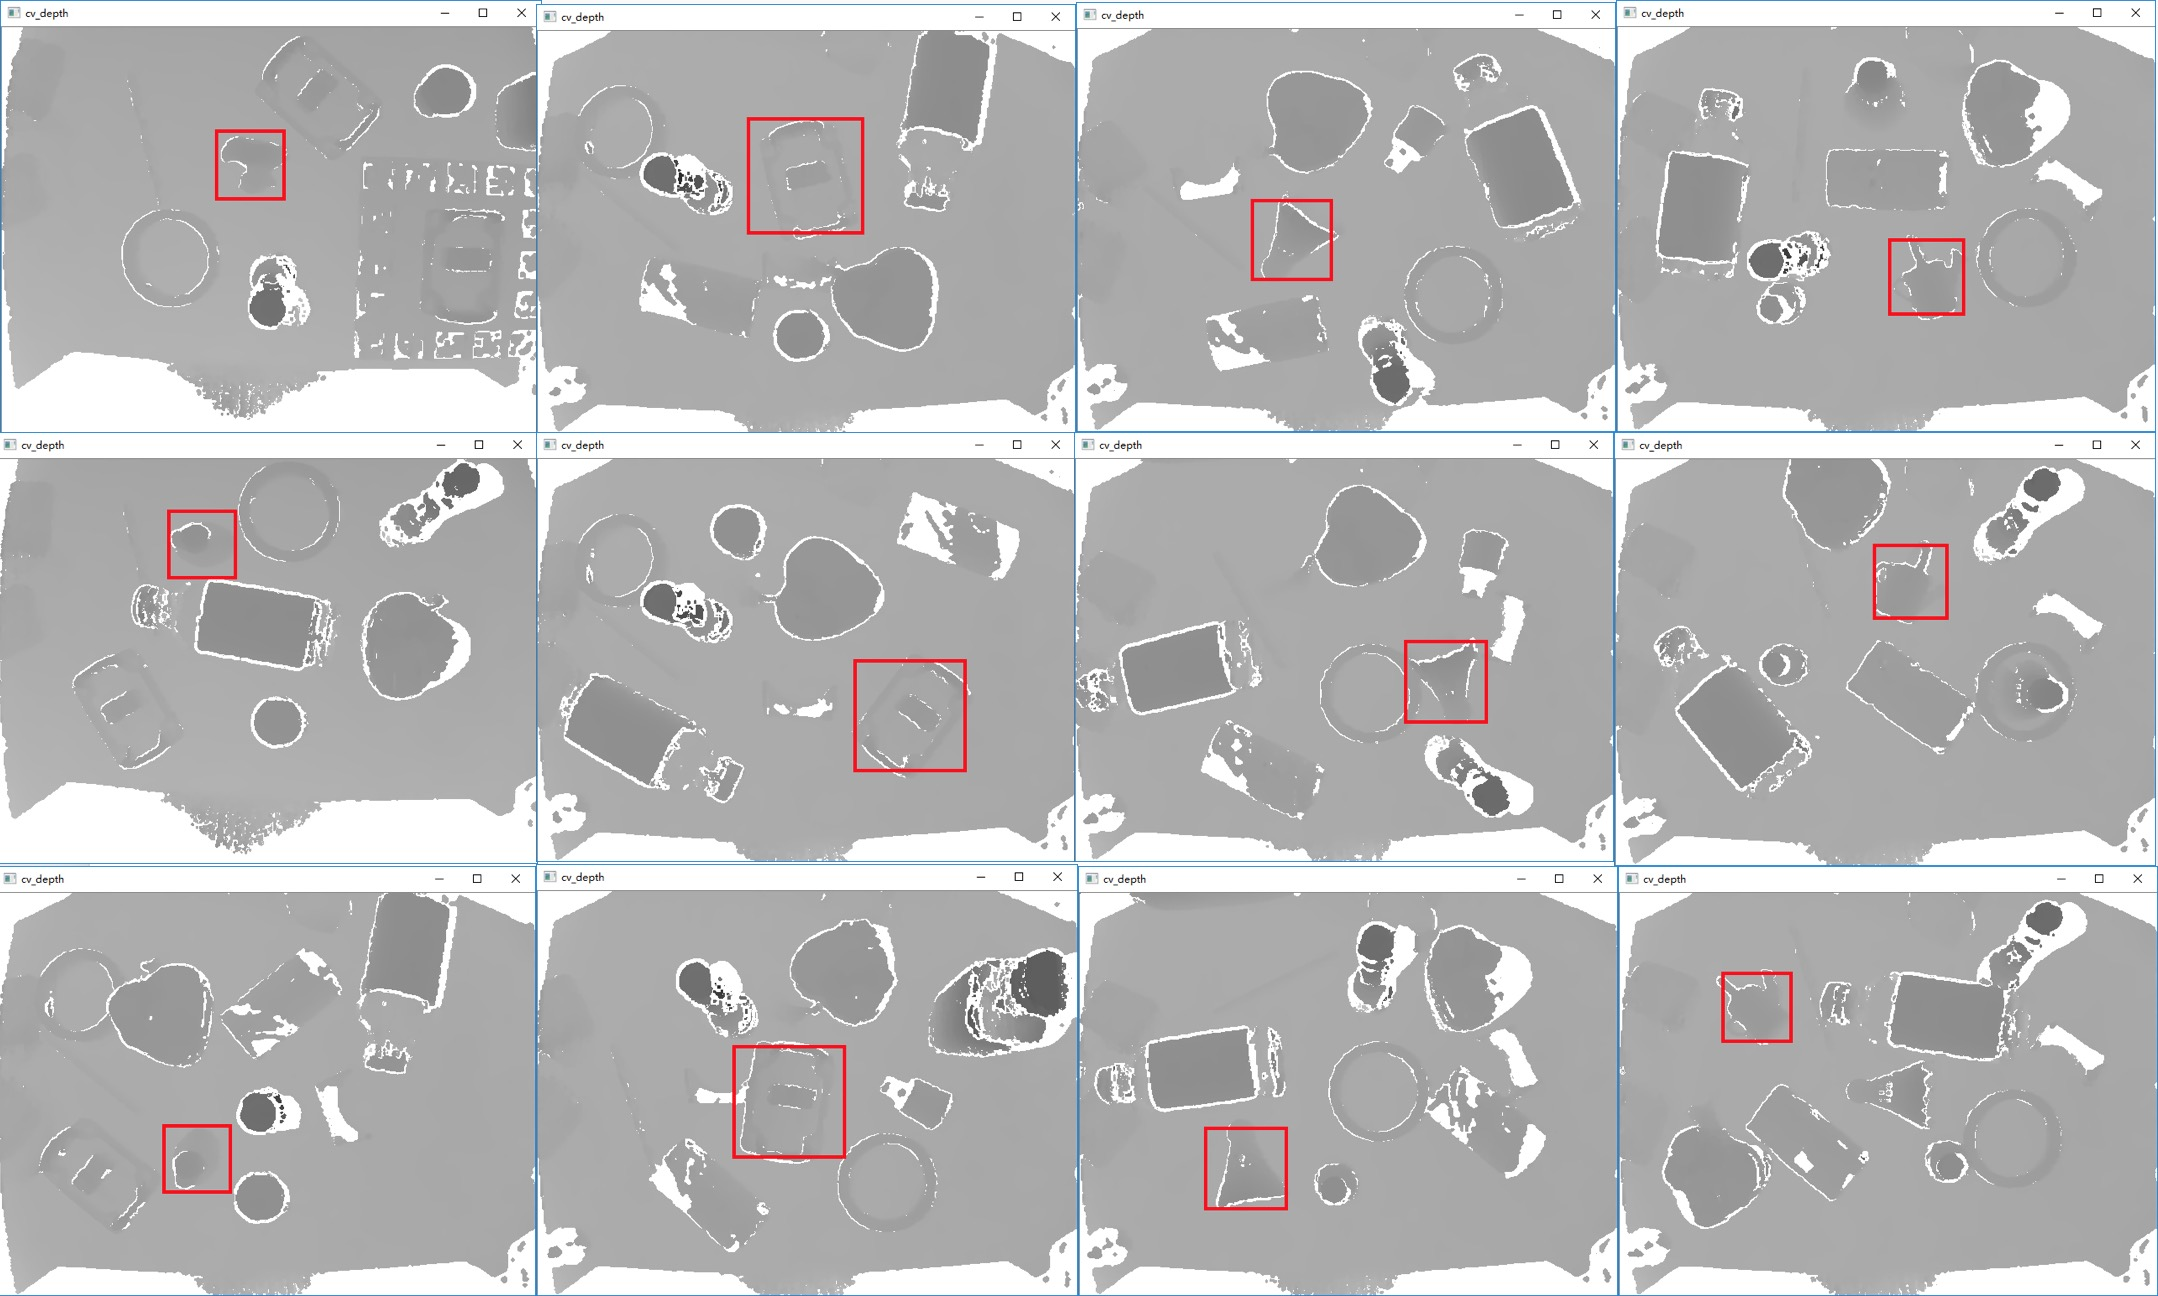
\includegraphics[width=\textwidth]{./mypic/物体检测结果图.jpg} 
	% \includegraphics[scale=1.0]{./cyk/test.jpg} 
	\caption{物体检测结果示意图} 
\end{figure}

\begin{table}[htb]
	\zihao{5}
	\caption{利用物体位姿估计特征进行物体检测实验} 
	% \label{Tabkeyword}
	\centering 
	\begin{tabular}[t]{
		% |c|l|r|p{4cm}|} 
		ccccccc} 
		\toprule
		物体类别 & 成功检测帧数 & 总帧数 & 查准率\\ 
		\midrule
		开关零件盒底座 & 1502 & 1524 & 98.56\% \\
		羽毛球模型 & 1664 & 1681 & 98.99\% \\
		小黄鸭模型 & 1542 & 1556 & 99.10\% \\
		水壶模型 & 1583 & 1604 & 98.69\% \\
		\bottomrule
	\end{tabular}
\end{table}



从表4-1可以看出,利用物体位姿估计特征进行物体检测在实验中4个样本物体上都取得了高于98\%的查准率,可见该方法的合理性。并且,经过复查,几乎所有的漏检案例中,导致分类器漏检的原因都是由于被检测物体在特定的角度下表面材质反光,在深度图像上形成了巨大的空洞,从而使提取到的特征严重失真。

但另一方面,本实验也有一定的不足之处。由于实验场所有限,背景信息并不复杂,干扰物少,使得分类器在区分前景和背景的过程中几乎没有困难,从而导致物体的查准率能够如此之高。但对于工业场景而言,该方法有足够的能力完成物体检测任务,毕竟在工业场景中不会出现非常复杂的背景。

\subsection{无遮挡情况下的物体六维位姿估计实验}

本文采用4.3节所述的位姿估计算法框架,在C++编程环境下实现了该算法。并通过自己制作了一套数据集对该算法进行了评估。

数据集主要包含真实物体在深度相机下各个朝向的位姿,以及对应位姿下深度相机采集到的深度图像数据,如图4-9所示。不像仿真环境数据可以直接获取物体在空间中的位姿,为了得到真实数据集中各个物体的真实位姿,本文采用ARTag技术协助标注真实位姿。如图4-8所示,将物体固定在ARTag标定板的中间,通过RGB相机可以方便的计算出ARTag板相对于相机的空间位姿,进一步空间坐标换算可以粗略的得到物体相对于深度相机坐标系下的位姿。在有了粗略的相对位姿后,可以通过将物体的3D模型反投影到对应的深度图像中,以点云的方式对物体的位姿进行微调最后得到精准的数据集样本。
\begin{figure}[htb]
	\centering 
	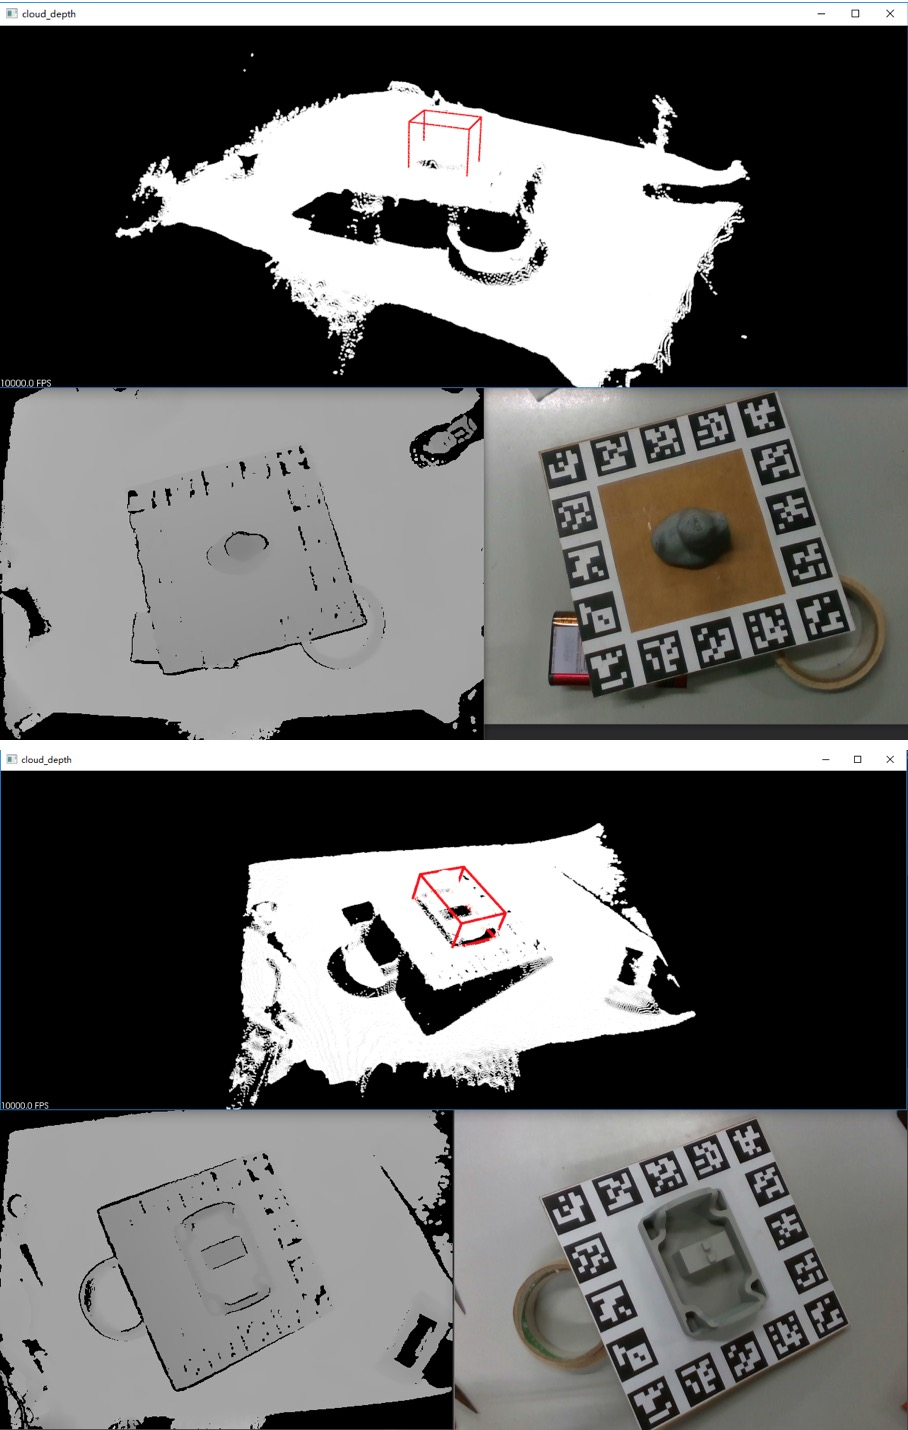
\includegraphics[width=0.7\textwidth]{./mypic/数据集制作2.jpg} 
	% \includegraphics[scale=1.0]{./cyk/test.jpg} 
	\caption{数据集制作示意图} 
\end{figure}

由于数据集制作过程中,单人完成一个目标物体每100个样本制作平均需要4到5天时间(包括3D模型制作、打磨、喷漆等环节),截止本文撰写时仅仅完成了急停开关零件盒底座的数据集制作,因此本文更多的实验数据来自于仿真环境给出的仿真数据。

在真实数据集上测试的效果如表4-2所示,其中数据集内含标注样本数量487个,着重与文章[\citenum{drost2010model}]中的方法进行了比较。其中文章[\citenum{drost2010model}]采用的方法为先通过投票法计算深度图像中的局部特征点与3D文件中的特征点匹配关系,计算得到初始位姿后利用ICP算法进行进一步调优得到最终位姿估计结果。本实验在仿真数据集上进行测试的效果如表4-3所示,其中数据集包含7种物体,每种物体样本数量为500个。
\begin{table}[htb]
	\zihao{5}
	\caption{真实数据集上测试的位姿估计精度表现} 
	% \label{Tabkeyword}
	\centering 
	\begin{tabular}[t]{
		% |c|l|r|p{4cm}|} 
		ccc} 
		\toprule
		方法类别 & 本方法 & 文章[\citenum{drost2010model}]\\ 
		\midrule
		X方向平移误差(单位:mm) & 1.35 & 0.59\\
		Y方向平移误差(单位:mm) & 0.83 & 0.71\\
		Z方向平移误差(单位:mm) & 1.95 & 1.41\\
		X方向欧拉角误差(单位:度) & 2.30 & 1.85\\
		Y方向欧拉角误差(单位:度) & 1.31 & 2.25\\
		Z方向欧拉角误差(单位:度) & 1.13 & 3.36\\
		\midrule
		失败率 & 0\% & 67.4\% \\
		\midrule
		算法速度 & 30fps & 0.46fps \\
		\bottomrule
	\end{tabular}
\end{table}

\begin{table}[htb]
	\zihao{5}
	\caption{仿真数据集上测试的位姿估计精度表现} 
	% \label{Tabkeyword}
	\centering 
	\begin{tabular}[t]{
		% |c|l|r|p{4cm}|} 
		cccccccc} 
		\toprule
		物体类别 & 开关零件盒底座 & 开关零件头 & 羽毛球 & 小黄鸭 & 水壶 & 茶杯 & 相机\\ 
		\midrule
		X方向平移误差(单位:mm) & 1.13 & 0.97 & 0.99& 1.30& 1.16&1.22 &1.06 \\
		Y方向平移误差(单位:mm) & 0.78 & 0.81 & 1.16&1.05 &1.19 &1.02 &1.15 \\
		Z方向平移误差(单位:mm) & 0.95 & 1.02 & 1.08& 1.08& 0.97& 1.30&1.20 \\
		X方向欧拉角误差(单位:度) & 1.81 & 1.55 &1.30 &1.09 &1.98 &1.76 &1.15 \\
		Y方向欧拉角误差(单位:度) & 1.11 & 1.01 &1.40 &1.27 &1.50 &1.24 &1.82 \\
		Z方向欧拉角误差(单位:度) & 1.03 & 1.38 &1.16 &1.38 &1.13 &1.59 &1.60 \\
		\bottomrule
	\end{tabular}
\end{table}

从表4-2中可以看出,本文提出的方法在物体位姿估计的精度上相比文章[\citenum{drost2010model}]要稍显不足,主要表现在质心空间坐标的位姿估计精度不够以及X方向欧拉角误差较高。但相比于文章[\citenum{drost2010model}],本文提出的方法具有两个重大优势,第一点在于本文方法的失败率极低,能够应对绝大多数情况下的位姿估计问题,而文章[\citenum{drost2010model}]则由于算法上的缺陷,有67.4\%情况下无法得到物体的位姿结果。第二点在于算法的效率,本文方法借助高效的特征描述以及随机蕨级联回归框架能够达到每秒处理30帧数据的速度,做到实时物体位姿估计,这是文章[\citenum{drost2010model}]无法做到的。

对比表4-2与表4-3,可以发现在真实数据集上测试的效果与仿真数据集上测试的效果差别并不大,这一点表明了仿真环境得到的深度图像数据与真实环境中的差别已经很小了。同时,表4-3中7个物体的位姿估计精度差别也都保持着非常接近的数据,这表明了本文所提的这套级联位姿估计算法框架的合理性以及通用性。图4-9展示了一些真实数据集上的位姿估计可视化结果,其中绿色方框表示物体位姿的真值,红色方框表示物体的位姿估计结果。

\begin{figure}[htb]
\centering 
\subfigure[]{\label{fig:subfig:a}
		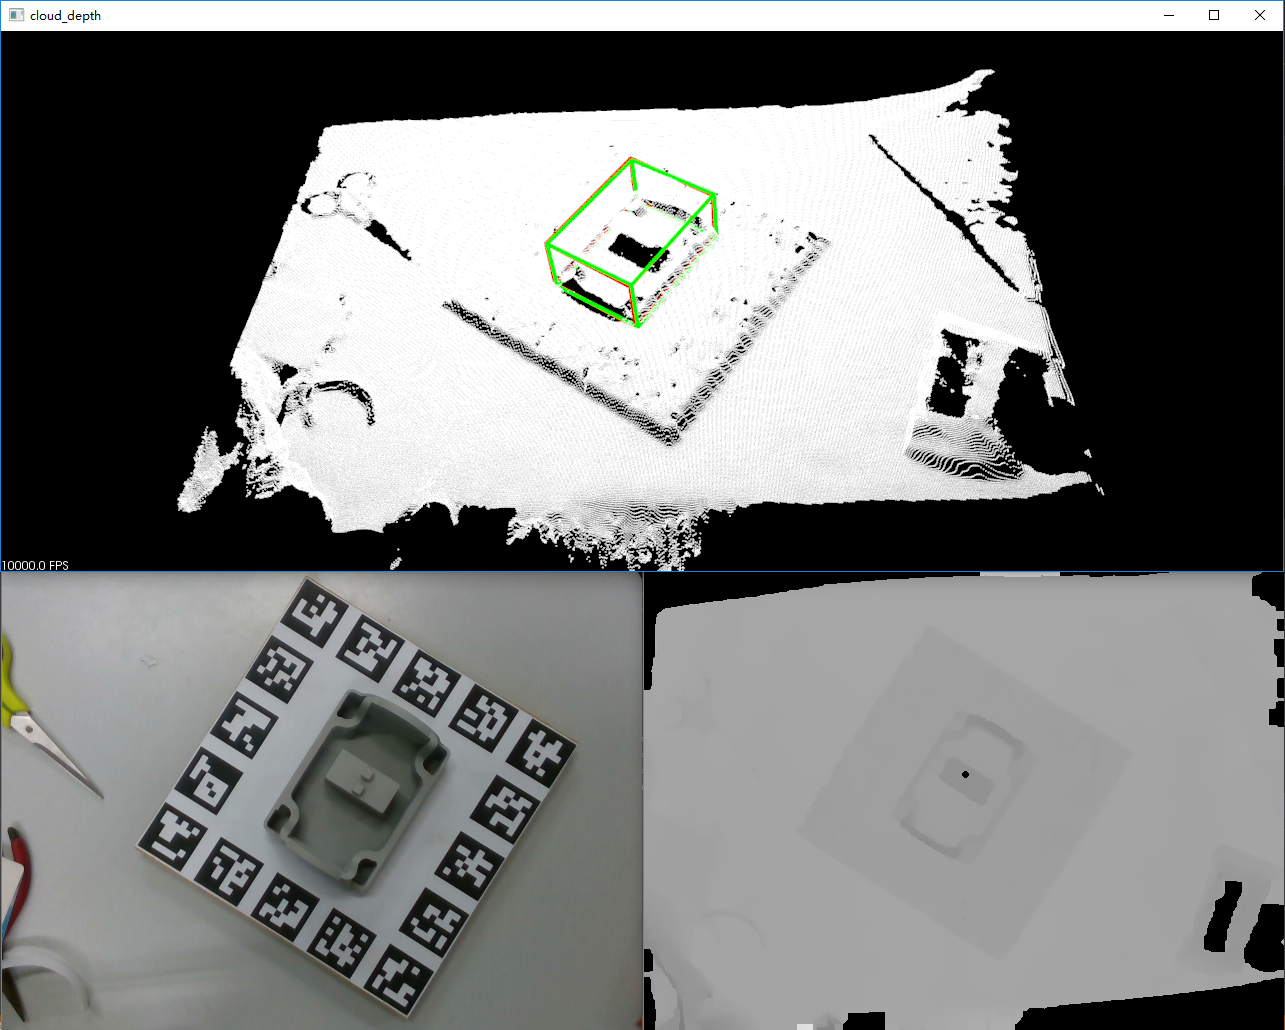
\includegraphics[width=0.4\linewidth]{./mypic/94.png} 
% \includegraphics[width=0.4\linewidth]{losebg_small}
}
\hspace{0.01\linewidth}
\subfigure[]{\label{fig:subfig:b}
		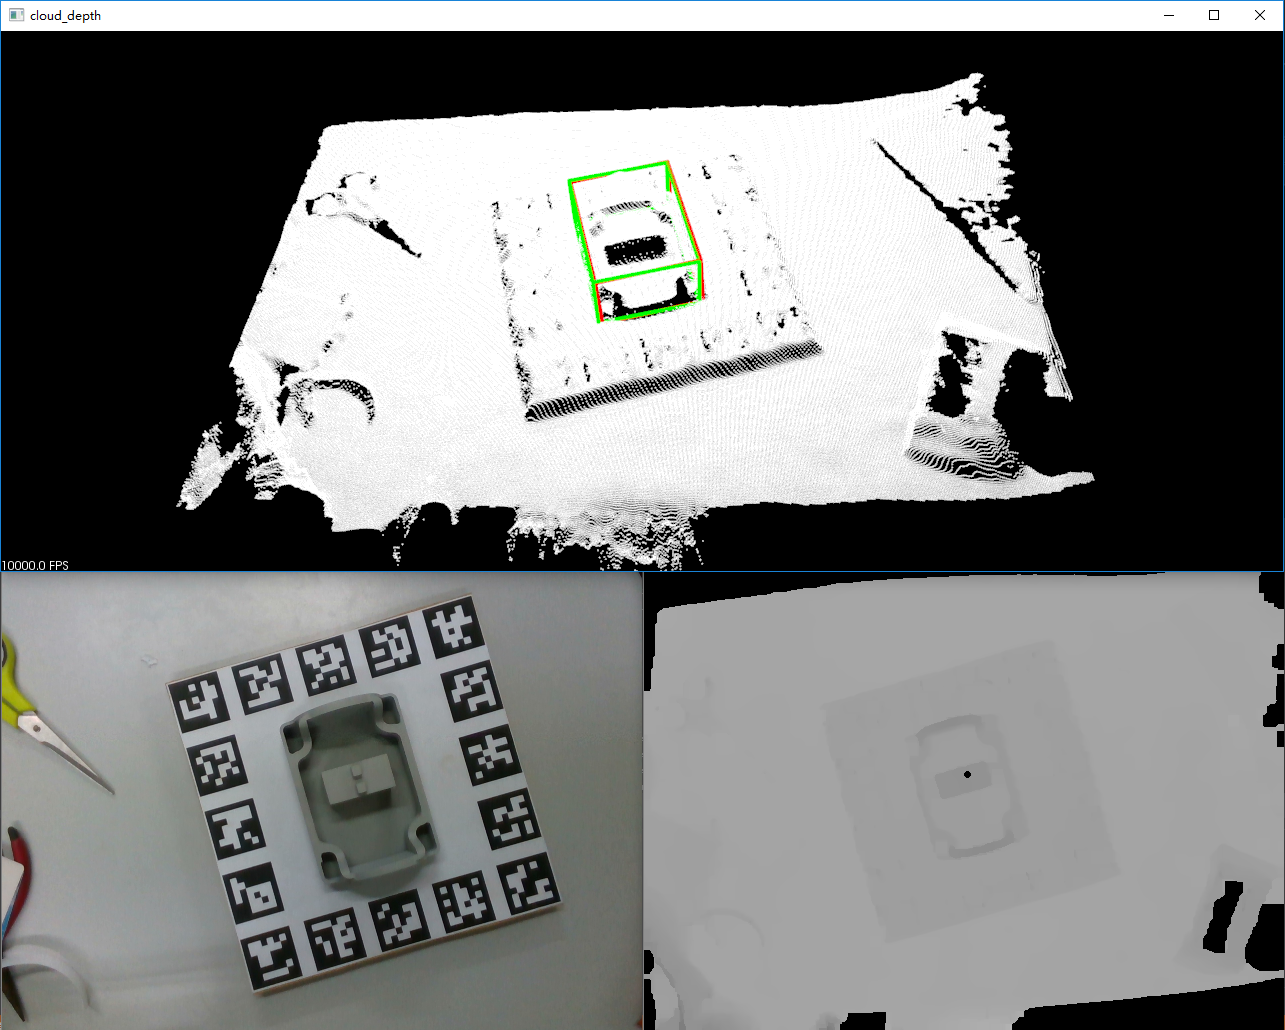
\includegraphics[width=0.4\linewidth]{./mypic/95.png} 
% \includegraphics[width=0.4\linewidth]{losebg_small}
}
\vfill
\subfigure[]{\label{fig:subfig:a}
		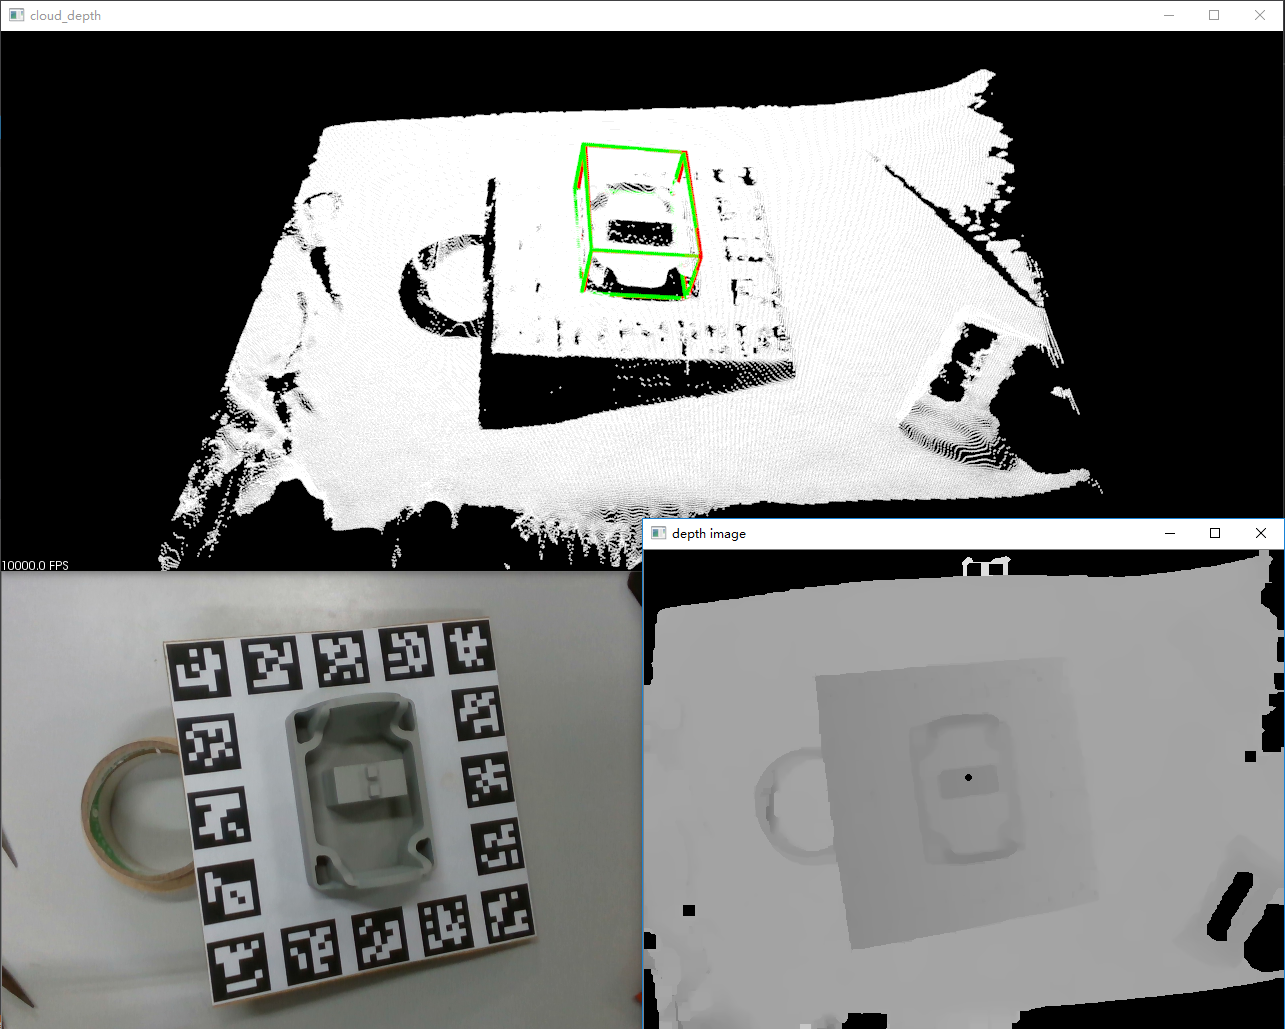
\includegraphics[width=0.4\linewidth]{./mypic/96.png} 
% \includegraphics[width=0.4\linewidth]{losebg_small}
}
\hspace{0.01\linewidth}
\subfigure[]{\label{fig:subfig:b}
		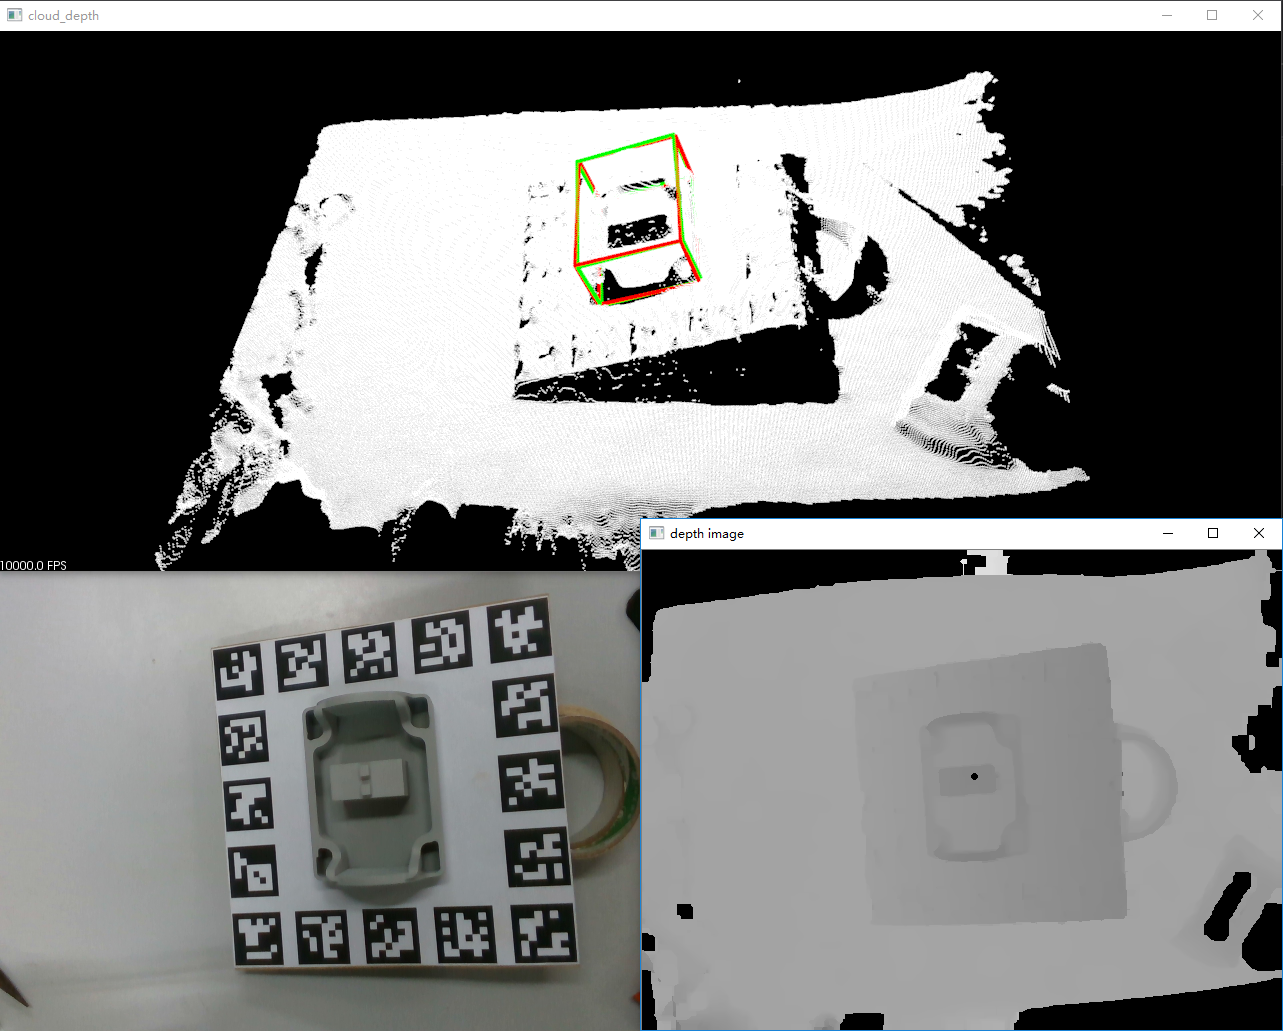
\includegraphics[width=0.4\linewidth]{./mypic/98.png} 
% \includegraphics[width=0.4\linewidth]{losebg_small}
}
\vfill
\subfigure[]{\label{fig:subfig:a}
		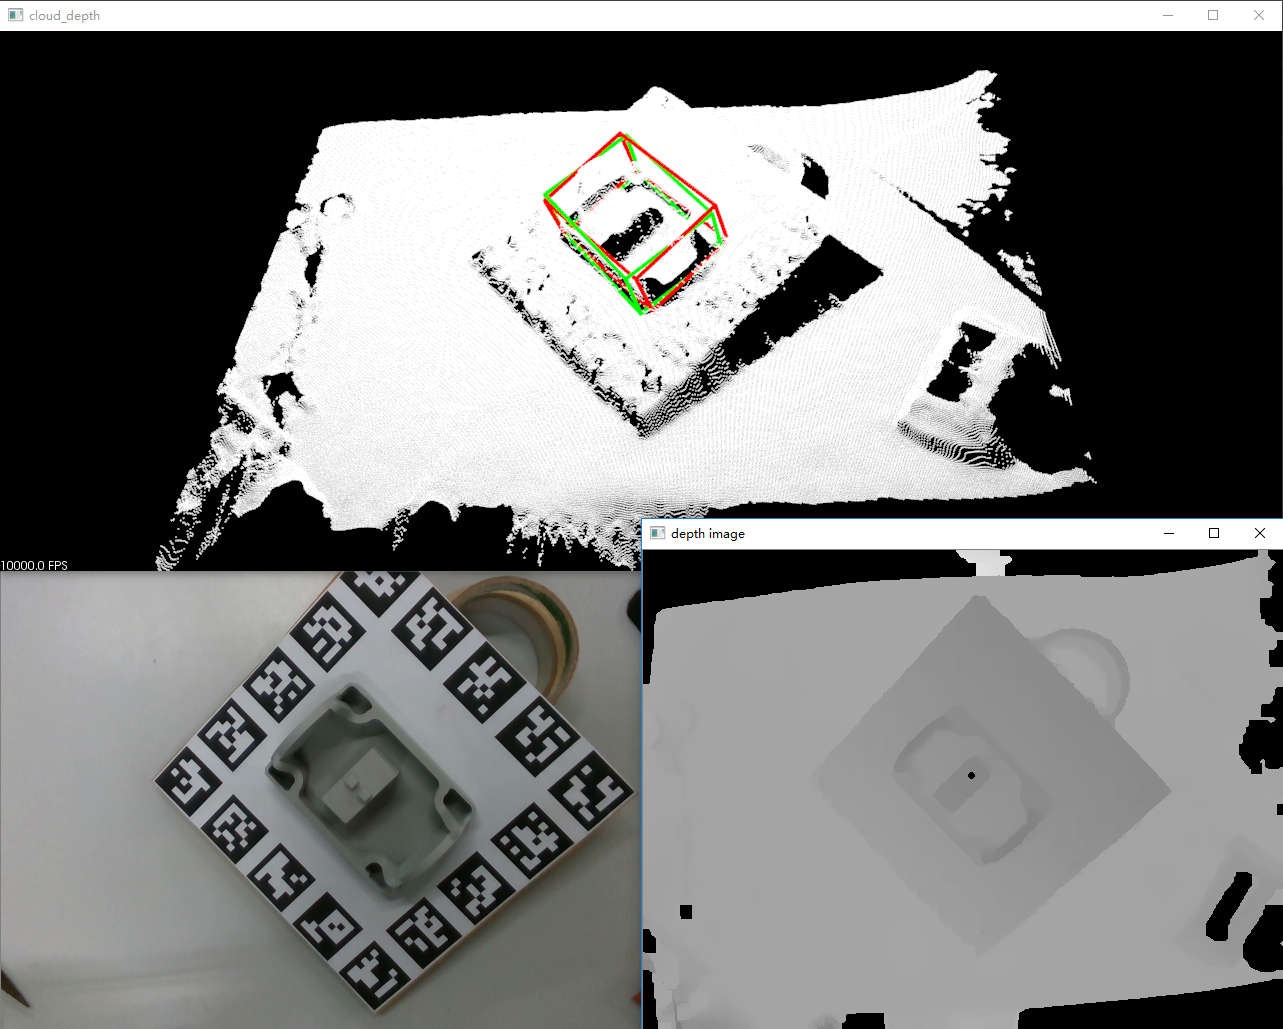
\includegraphics[width=0.4\linewidth]{./mypic/99.png} 
% \includegraphics[width=0.4\linewidth]{losebg_small}
}
\hspace{0.01\linewidth}
\subfigure[]{\label{fig:subfig:b}
		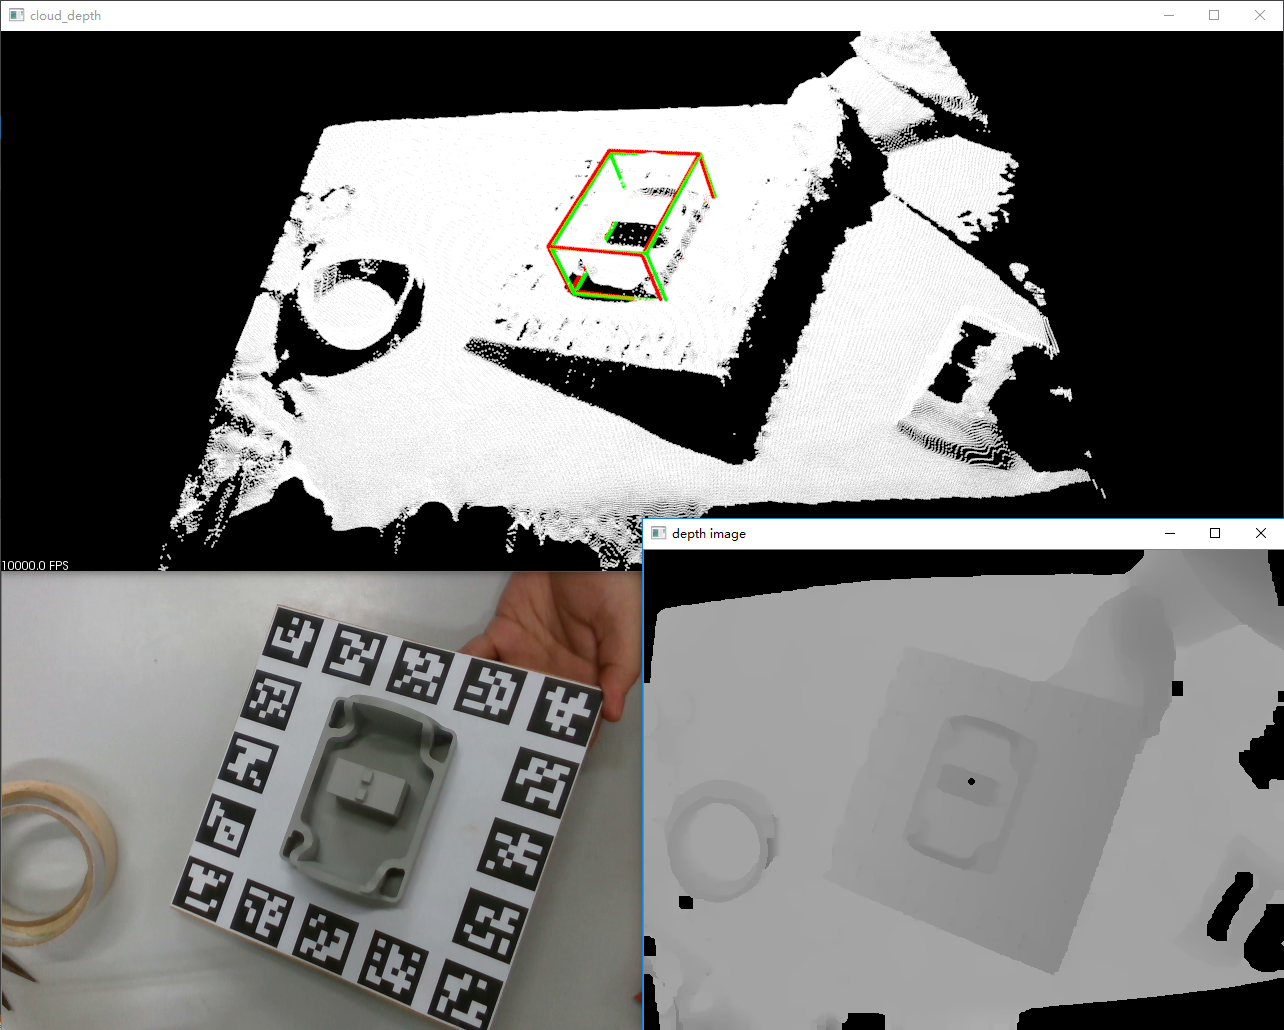
\includegraphics[width=0.4\linewidth]{./mypic/100.png} 
% \includegraphics[width=0.4\linewidth]{losebg_small}
}
\caption{一些真实数据集上的位姿估计可视化结果}
% \label{fig:subfig}
\end{figure}

\newpage

\subsection{有遮挡情况下的物体六维位姿估计实验}

本文根据4.4节内容所提方法进一步改进物体六维位姿估计算法,对物体被遮挡时的位姿估计进行了实验。首先验证了是否能够通过原始特征拿到物体当前状态下被遮挡的情况,本文采用经典随机蕨分类器作为基本工具,采用第三章所提的仿真数据训练了一个遮挡情况预测器。如图4-10所示,在零件周围随机撒点,预测器能够顺利预测出物体被遮挡的情况,在图中被遮挡的位置用绿色点标出。
\begin{figure}[htb]
	\centering 
	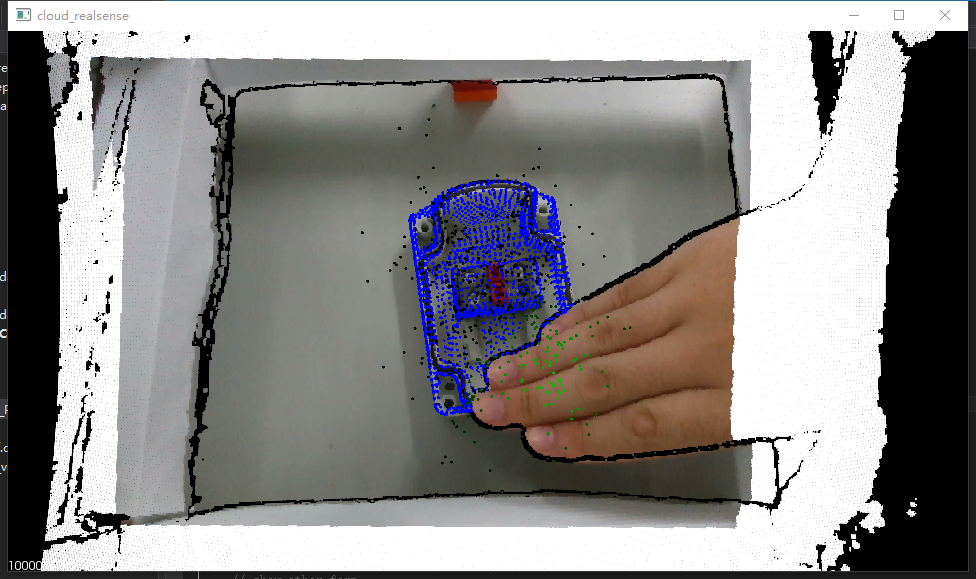
\includegraphics[width=0.7\textwidth]{./mypic/1.png} 
	% \includegraphics[scale=1.0]{./cyk/test.jpg} 
	\caption{利用简单的随机蕨分类器对物体的被遮挡情况进行估计} 
\end{figure}

在得到物体的被遮挡情况之后,便可以套用4.4节整体算法框架进行实验。实验设定与4.6.2节所述相似,本节将不再重复叙述。实验结果如表4-4以及表4-5所示,其中真实数据集样本数量为328个,仿真数据集样本数量为5000个。

\begin{table}[htb]
	\zihao{5}
	\caption{真实数据集上测试的位姿估计精度表现(有遮挡)} 
	% \label{Tabkeyword}
	\centering 
	\begin{tabular}[t]{
		% |c|l|r|p{4cm}|} 
		cccc} 
		\toprule
		方法类别 & \makecell[c]{本方法\\(采用遮挡情况估计策略)} & 文章[\citenum{drost2010model}] & \makecell[c]{本方法\\(不采用遮挡情况估计策略)}\\ 
		\midrule
		X方向平移误差(单位:mm) & 1.58 & 5.95 & 12.64\\
		Y方向平移误差(单位:mm) & 1.46 & 3.43 & 10.93\\
		Z方向平移误差(单位:mm) & 2.55 & 10.2 & 5.76\\
		X方向欧拉角误差(单位:度) & 3.91 & 1.34 & 8.65\\
		Y方向欧拉角误差(单位:度) & 4.17 & 5.01 & 11.08\\
		Z方向欧拉角误差(单位:度) & 4.02 & 2.00 & 8.61\\
		\midrule
		失败率 & 0\% & 73.1\% & \/\\
		\midrule
		算法速度 & 27fps & 0.46fps & \/ \\
		\bottomrule
	\end{tabular}
\end{table}

\begin{table}[htb]
	\zihao{5}
	\caption{仿真数据集上测试的位姿估计精度表现(有遮挡)} 
	% \label{Tabkeyword}
	\centering 
	\begin{tabular}[t]{
		% |c|l|r|p{4cm}|} 
		cccccccc} 
		\toprule
		物体类别 & 开关零件盒底座 & 开关零件头 & 羽毛球 & 小黄鸭 & 水壶 & 茶杯 & 相机\\ 
		\midrule
		X方向平移误差(单位:mm) &1.50&2.27&1.57&1.96&1.99&1.53&1.96 \\
		Y方向平移误差(单位:mm) & 1.97 & 2.08 & 2.05&1.76&1.75&2.26&1.40 \\
		Z方向平移误差(单位:mm) &1.60&1.50&1.23&1.87&1.41&1.79&1.63 \\
		X方向欧拉角误差(单位:度) &3.54&4.48&3.94&4.13&5.07&4.65&4.65 \\
		Y方向欧拉角误差(单位:度) &3.76&4.47&4.11&3.27&3.95&3.81&3.60 \\
		Z方向欧拉角误差(单位:度) &4.60&3.79&4.43&4.32&4.71&3.55&3.26 \\
		\bottomrule
	\end{tabular}
\end{table}

对比表4-2和表4-4以及对比表4-3和表4-5不难发现,在有遮挡情况下本文所提方法和文章[\citenum{drost2010model}]在位姿回归精度上都有下降。但于此同时,对比表4-3中第2列和第3列可以看出,本文方法在质心空间坐标上的估计精度远高于文章[\citenum{drost2010model}],并且在Y方向欧拉角误差也略高于文章[\citenum{drost2010model}]。对比表4-3中第2列和第4列可以得到,采用了遮挡情况估计策略能够大大提高物体位姿估计算法的鲁棒性。可以认为如果本文所提的级联位姿估计算法如果没有遮挡情况估计策略,是无法对被局部遮挡的物体进行位姿估计的。这也间接证实了2.3节所提的大噪声干扰下的随机蕨回归算法的合理性。此外,采用了遮挡情况估计策略会略微降低算法的计算效率,但仍然能够满足实时位姿估计。

\begin{figure}[htb]
	\centering 
	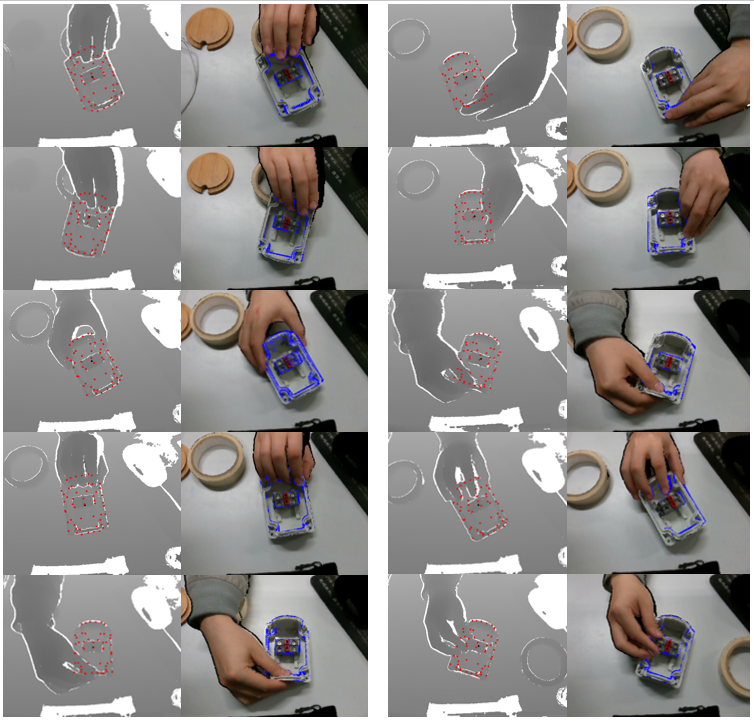
\includegraphics[width=0.9\textwidth]{./mypic/71.png} 
	% \includegraphics[scale=1.0]{./cyk/test.jpg} 
	\caption{一些真实场景下有遮挡情况的物体位姿估计结果} 
\end{figure}

图4-11给出了一些真实场景下有遮挡情况的物体位姿估计结果,图中红点和蓝点分别表示深度图像下和点云图下的位姿估计结果的模型重投影。可以看出重投影后的物体模型与实际数据都能保持较好的重合率,表明本文算法的合理性。



\section{本章小节}

本章利用第2章以及第3章做好的铺垫,设计并利用随机蕨级联回归框架开发出一套完整的物体位姿估计方案。该位姿估计方案提出了一种针对深度图像的具有尺度不变性的特征描述,并通过合理分配不同层级的回归目标,实现了位姿估计算法的高效性、实时性。同时,针对存在遮挡情况的物体位姿估计问题,本章利用改进后的随机蕨算法提出了一套具有更高鲁棒性的位姿估计算法框架。最后还充分利用整个算法框架中的富余特征信息进行物体初始位置检测,实现了一个更为完整的端到端物体位姿估计方案。通过实验,上述方案的可行性都得到了一定程度的证实。













